\documentclass[11pt,a4paper]{article}
\newcommand{\guideshort}{Detailed user guide}
% Shared typesetting for the two source-grounded VGAI teaching guides.
\usepackage[a4paper,margin=23mm,headheight=15pt]{geometry}
\usepackage{fontspec}
\setmainfont{Liberation Serif}
\setsansfont{Liberation Sans}
\setmonofont{Liberation Mono}
\usepackage{xcolor,graphicx,booktabs,tabularx,longtable,array}
\usepackage{listings,hyperref,tikz}
\usetikzlibrary{arrows.meta,positioning}
\definecolor{vveblue}{HTML}{174A70}
\definecolor{vvelight}{HTML}{F1F5F8}
\definecolor{vvegreen}{HTML}{266547}
\hypersetup{colorlinks=true,linkcolor=vveblue,urlcolor=vveblue,
  pdfauthor={Vienna Game AI Library},pdfsubject={Source-grounded beginner teaching edition}}
\setlength{\parindent}{0pt}
\setlength{\parskip}{6pt plus 1pt}
\setlength{\emergencystretch}{3em}
\sloppy
\renewcommand{\arraystretch}{1.18}
\makeatletter
\def\ps@vve{%
  \def\@oddhead{\small\sffamily Vienna Game AI Library\hfil\guideshort}%
  \let\@evenhead\@oddhead
  \def\@oddfoot{\small\sffamily Teaching edition / 16 October 2026\hfil\thepage}%
  \let\@evenfoot\@oddfoot}
\makeatother
\pagestyle{vve}
\lstdefinestyle{vvecpp}{language=C++,basicstyle=\ttfamily\small,
  keywordstyle=\color{vveblue}\bfseries,commentstyle=\color{vvegreen},
  stringstyle=\color{vvegreen},backgroundcolor=\color{vvelight},
  breaklines=true,breakatwhitespace=false,columns=fullflexible,
  keepspaces=true,showstringspaces=false,tabsize=4,
  frame=single,rulecolor=\color{vvelight},framesep=6pt,
  xleftmargin=6pt,xrightmargin=6pt,aboveskip=8pt,belowskip=8pt,
  morekeywords={import,requires,concept,constexpr,consteval,nodiscard}}
\lstset{style=vvecpp}
\newcommand{\api}[1]{{\ttfamily\small\detokenize{#1}}}
\newcommand{\source}[1]{\par\smallskip{\raggedright\footnotesize\sffamily\color{vveblue}Source: \nolinkurl{#1}.\par}}
\newcommand{\lesson}[1]{\clearpage\section{#1}}
\newenvironment{remember}{\begin{quote}\small\textbf{Remember. }}{\end{quote}}
\newenvironment{tryit}{\begin{quote}\small\textbf{Try it. }}{\end{quote}}
\newcommand{\guidecover}[3]{%
 \begin{titlepage}\sffamily\color{vveblue}
 {\large Vienna Game AI Library\par}\vspace{20mm}
 {\Huge\bfseries #1\par}\vspace{8mm}
 {\Large #2\par}\vspace{12mm}
 \color{black}{\large #3\par}\vfill
 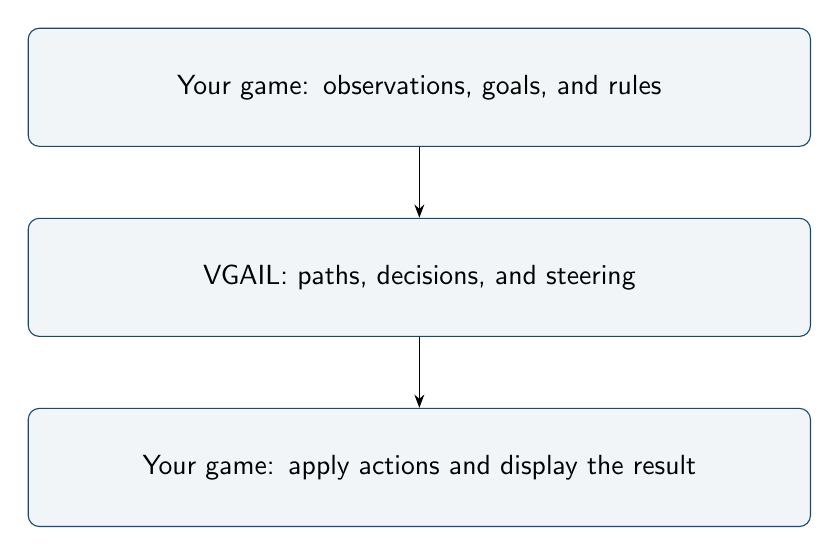
\begin{tikzpicture}[node distance=9mm,every node/.style={draw=vveblue,rounded corners,fill=vvelight,text width=0.8\linewidth,align=center,minimum height=15mm,font=\sffamily}]
 \node (game) {Your game: observations, goals, and rules};
 \node (engine) [below=of game] {VGAIL: paths, decisions, and steering};
 \node (result) [below=of engine] {Your game: apply actions and display the result};
 \draw[-{Stealth}] (game)--(engine);
 \draw[-{Stealth}] (engine)--(result);
 \end{tikzpicture}\vfill
 {\normalsize Updated 16 October 2026\par}
 {\small Source baseline: b1c76a1.\par}
 {\small Complete examples are checked against this source; excerpts state their context.\par}
 \end{titlepage}}

\hypersetup{pdftitle={Vienna Game AI Library - Detailed user guide}}
\begin{document}
\guidecover{Detailed user guide}{Game AI explained from the first concepts}{Learn how route finding, state machines, decision trees, steering, flocking and Monte Carlo tree search work together. Includes complete console programs and practical integration limits.}
\tableofcontents
\lesson{How to read this guide}
This is a practical introduction to the Vienna Game AI Library, abbreviated VGAI. It follows the source in commit \api{b1c76a1}, checked on 16 October 2026. The public namespace is \api{VGAIL}. The single header is \api{ViennaGameAILibrary.hpp}. Examples use C++20 and small console programs so you can see an algorithm's behaviour before adding a renderer.

Read the opening sections if game AI is new to you. Then choose the part matching your next feature: routes, state machines, decision trees, steering, flocking or Monte Carlo tree search. Each part explains the problem first, introduces vocabulary, shows the actual API and describes what your game must supply.

A complete listing includes \api{main} and its standard headers. A fragment is explicitly described as such. The complete examples return nonzero on a failed check and print named results. They check the lesson's claim; they do not prove that every algorithm is correct for every possible game.

This library is an educational collection. Some names resemble larger engine facilities but have narrower meanings here. For example, \api{NavMesh} is a grid, and a \api{Boid} does not provide a collision engine. The guide explains current behaviour so your game can make appropriate decisions.
\lesson{What game AI means here}
Game AI is code that chooses what a game-controlled character or system should do. A guard might patrol, notice a player, find a route and move along it. Those are different decisions at different scales. Choosing chase is a behaviour decision. Choosing a corridor is route planning. Turning toward the next point is local movement.

This library uses explicit algorithms and rules. It does not train a neural network or call a language model. The word intelligent describes the useful behaviour the player sees, not a promise of human reasoning. A small rule can produce a clear, convincing response when the game supplies sensible information.

The game supplies perception: whether an enemy is visible, where walls are, how much health remains and which actions are legal. VGAI does not inspect a rendered image or discover those facts automatically. A renderer shows the result, and a physics or collision system decides which proposed movements are allowed.

Keep these responsibilities clear when debugging. If an agent chooses chase correctly but walks through a wall, the state machine may be working. The movement or collision layer may need attention. If its route is valid but it follows the wrong waypoint, inspect the route follower rather than rewriting A*.
\lesson{A map of the library}
\textbf{Pathfinding}: \api{NavMesh}, \api{NodeData}, \api{Vec2ui} and related helpers represent a grid and search routes. Start here when an agent needs to navigate around blocked cells.

\textbf{State machines}: \api{StateMachine}, \api{State} and transitions hold a current activity and change it when a condition becomes true. Use them for behaviours such as patrol, chase and return.

\textbf{Decision trees}: \api{DecisionTree} and \api{DecisionNode} give you an owned tree. Your derived node classes decide which child to call or which action to perform.

\textbf{Steering and flocking}: \api{Vec2f}, \api{Boid} and \api{Flock} calculate and apply two-dimensional movement. Local rules influence velocity; they do not supply a complete collision controller.

\textbf{Monte Carlo tree search}: \api{Action}, \api{MCTSState}, \api{MCTSNode} and \api{MCTS} explore copied game states through trial actions. You define the state, the legal actions and how a game ends.

The repository's Demo uses raylib for graphics. The algorithms in these console examples use no raylib calls. The top-level CMake adds the Demo unconditionally, so a small separate console project is the clearest first integration.
\source{include/ViennaGameAILibrary.hpp; Demo/CMakeLists.txt}
\lesson{The C++ ideas you need}
A class groups data and functions. An object is one instance of that class. \api{VGAIL::NavMesh map(8,6,0.0f);} creates a map object with constructor arguments. The \api{::} selects a name from a namespace or class. A member call such as \api{map.findPath(...)} asks that object to do work.

A \api{std::vector<T>} is a growable sequence of values. Its first element has index zero. A pointer stores an address; \api{auto* state} is a pointer whose type the compiler deduces. A reference, written \api{T&}, is another way to refer to an existing object. Neither a pointer nor a reference automatically owns the object it names.

A lambda is a small function you write where you need it. The syntax \api{[&] { return enemyNear; }} captures local variables by reference, so it sees their current values when called. That is useful for live game conditions, provided the referenced variables are still alive.

A virtual function lets a derived class supply behaviour through a base-class interface. The decision-tree examples derive from \api{DecisionNode} and override \api{makeDecision}. The tree owns those nodes and calls their functions; your class provides their meaning.

A template is code parameterized by types. \api{MCTS<Turn,Move>} specializes the search for your game's state and action types. It cannot infer game rules from those names; those types must offer the operations the search uses.
\lesson{Build a console exercise}
Use a C++20 compiler and its standard library. The library uses \api{std::jthread} in its MCTS code, so a compiler that accepts only older C++ modes is insufficient even if you begin with pathfinding. Link threading support as your platform requires.

Create a folder beside the library checkout. Put one complete example in \api{main.cpp} and use this build file:\begin{lstlisting}
cmake_minimum_required(VERSION 3.20)
project(FirstAI LANGUAGES CXX)
find_package(Threads REQUIRED)
add_executable(first_ai main.cpp)
target_compile_features(first_ai PRIVATE cxx_std_20)
target_compile_definitions(first_ai PRIVATE NDEBUG)
target_include_directories(first_ai PRIVATE
    ../ViennaGameAILibrary/include)
target_link_libraries(first_ai PRIVATE Threads::Threads)
\end{lstlisting}
Configure, build and run:\begin{lstlisting}
cmake -S . -B build -DCMAKE_BUILD_TYPE=Release
cmake --build build
./build/first_ai
\end{lstlisting}
With a multi-configuration generator, add \api{--config Release} and use its Release executable directory. Direct compilation is also possible with \api{c++ -std=c++20 -DNDEBUG -pthread -I../ViennaGameAILibrary/include main.cpp -o first_ai}.

The standard headers before the library include supply declarations the current header uses indirectly. \api{NDEBUG} selects the release assertion path, avoiding the Windows-specific debug-break intrinsic on Linux. It also disables those assertions, so validate sizes, indices and other preconditions explicitly in your application.

Start with one source file. Non-inline free-function definitions in the current header can create duplicate link symbols when several source files include it. For a larger game, place VGAI-dependent code in a dedicated integration source file and expose game-level functions from your own header.
\source{CMakeLists.txt; include/ViennaGameAILibrary.hpp: VGAIL_ASSERT and free functions}
\lesson{Build the graphical Demo later}
The Demo is useful once a console exercise works. It adds a window, drawing and interactive inputs, which help show routes or flock motion but also introduce more build dependencies. Read \api{Demo/CMakeLists.txt} to see which demo source is currently selected. In this source snapshot it selects flocking; an older README description of a default demo may differ.

Initialize the raylib submodule before using the top-level build:\begin{lstlisting}
git submodule update --init --recursive
cmake -S . -B build -DCMAKE_BUILD_TYPE=Release
cmake --build build
\end{lstlisting}
These commands run from the VGAI repository root. The top-level project requires CMake 3.28. Platform window-system and graphics prerequisites come from raylib's build requirements. Doxygen is optional for API documentation; it is not required for the separate console project.

If configuration fails in the graphical route, first check that the submodule has its files and that your compiler, C++20 mode and platform graphics dependencies are available. Keep the console example working while resolving graphics setup. That gives you a small known-good reference for the library API.
\source{CMakeLists.txt; Demo/CMakeLists.txt; .gitmodules; README.md}
\lesson{Coordinates, vectors and elapsed time}
\api{Vec2ui} stores two unsigned integers. It is appropriate for grid-cell coordinates. A width of 8 gives valid x coordinates 0 through 7, not 1 through 8. The helper \api{getIndex} maps a cell to a linear position using x + y times width. Check bounds before using it; a calculated index is not proof that coordinates were valid.

\api{Vec2f} stores two floating-point numbers. It is used for continuous positions, velocities and directions. A velocity of \api{Vec2f{2,0}} means two world units per second along x if your game chooses those units. A direction says where to point; its magnitude says how long the vector is.

Use one agreed world scale. For example, make a grid cell one metre wide and put its centre at origin plus \api{(x+0.5,y+0.5)} times cell size. A screen coordinate system may point y downward; a top-down world drawn in 3D may use x and z instead. Your integration chooses that mapping, consistently in both directions.

Update durations for states and movement are seconds. A tenth of a second is 0.1, not 100. MCTS is a special case: its search budget argument is milliseconds. Keep the variable names explicit, such as \api{elapsedSeconds} and \api{searchBudgetMs}, to avoid a thousandfold unit error.
\clearpage\part{Finding and following routes}\lesson{What a route search solves}
A route search answers: which sequence of allowed cells connects this start to this target? It does not move the agent. It does not choose whether the target is sensible. It does not know the width of your character unless you account for that width in the map.

Represent a room or level as walkable cells and blocked cells. A blocked cell means the agent must not occupy it. If a character is wider than a point, block extra nearby cells or choose a suitable grid scale so a computed centre route also leaves enough clearance.

The result is a sequence of cell coordinates. Convert those coordinates to world-space waypoints and move toward the next one. When you arrive, advance to the following waypoint. If the target moves or the route becomes blocked, decide when to search again.

\begin{center}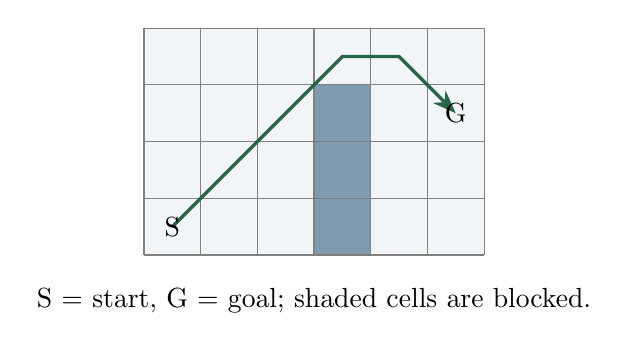
\begin{tikzpicture}[scale=0.72]
\fill[vvelight] (0,0) rectangle (6,4);
\foreach \y in {0,1,2} {\fill[vveblue!55] (3,\y) rectangle +(1,1);}
\draw[step=1cm,gray] (0,0) grid (6,4);
\draw[very thick,vvegreen,-{Stealth}] (0.5,0.5)--(1.5,1.5)--(2.5,2.5)--(3.5,3.5)--(4.5,3.5)--(5.5,2.5);
\node at (0.5,0.5) {S};\node at (5.5,2.5) {G};
\node[align=center] at (3,-0.8) {S = start, G = goal; shaded cells are blocked.};
\end{tikzpicture}\end{center}
This schematic shows a route around a barrier. Your returned route still needs a movement controller to follow it.

First test three cases without graphics: a clear route, a fully separating barrier, and start equal to target. Then draw the returned cells as markers. Comparing those markers with the collision map quickly reveals coordinate-system or indexing mistakes.
\lesson{Create a known map}
The grid constructor accepts width, height, obstruction fraction and optional region lengths. Use positive nonzero dimensions and positive region lengths. A zero obstruction fraction gives a known walkable grid. Then mark obstacles explicitly, which makes lessons and regression checks easier to repeat.\begin{lstlisting}
VGAIL::NavMesh map(8, 6, 0.0f);
map.setObstructable({3, 2});
map.setWalkable({3, 2});
\end{lstlisting}
The last two calls are fragments using the existing map. The public spelling is \api{setObstructable}. Check x and y against \api{getWidth()} and \api{getHeight()} before accessing a node or changing a cell. Avoid constructing huge maps before understanding their storage and preprocessing cost.

The obstruction argument supplies random map generation when nonzero. That is convenient for demonstrations, but a random map is a poor starting point for explaining a failure: the next run may create different obstacles. Store or explicitly construct the map used by a test.

Although its name says navigation mesh, this class is not an arbitrary polygon mesh over a 3D level. It builds grid nodes with up to eight neighbouring cells. Keep that distinction in mind when comparing it with navigation systems from larger game engines.
\source{include/ViennaGameAILibrary.hpp: NavMesh constructors; createRegions; NodeData}
\lesson{A complete route example}
% doc-example: vgai_path_manual
\begin{lstlisting}
#include <cfloat>
#include <cmath>
#include <cstdint>
#include <limits>
#include "ViennaGameAILibrary.hpp"

int main() {
    VGAIL::NavMesh map(8, 6, 0.0f);
    map.setObstructable({3, 2});
    auto path = map.findPath({0, 0}, {7, 5});
    const bool ok = !path.empty()
        && path.front() == VGAIL::Vec2ui{0, 0}
        && path.back() == VGAIL::Vec2ui{7, 5};
    std::cout << "path ok=" << ok
              << " cells=" << path.size() << '\n';
    for (const auto& p : path)
        std::cout << p.x << ',' << p.y << '\n';
    return ok ? 0 : 1;
}
\end{lstlisting}
The success check verifies the endpoints. The printed list lets you inspect intermediate cells. For a stronger regression check, verify every cell is in bounds and walkable and every pair of consecutive cells is adjacent. Compare route cost if your test is about optimality; do not require one exact route when equal-cost alternatives exist.
\lesson{Understand A star with a small choice}
A* ranks an unfinished route using two quantities. The first, often called g, is the cost already paid from the start. The second, h, estimates the cost still needed to reach the target. Their sum helps the search choose the next promising cell. These are bookkeeping values; they are not positions or velocities.

Suppose one possible next cell has cost-so-far 4 and estimated remainder 3. Its total estimate is 7. Another has cost-so-far 2 and estimated remainder 8, giving 10. The search prefers the first candidate now, even though the second was cheaper to reach. A wall may later change which candidate is best.

In this grid, straight and diagonal movement use geometric distances. A diagonal costs more than a horizontal step. The straight-line estimate helps guide the search without treating a diagonal as the same distance as a straight step. The algorithm records parents so it can reconstruct a route from the goal back toward the start.

Minimum cost and fewest cells are different goals when step costs differ. A route with a diagonal can cover more distance in fewer cell transitions. When testing, name the metric you care about. Preprocessed routing is a separate strategy with its own choices; do not assume every resulting route is globally shortest without testing the property you need.
\source{include/ViennaGameAILibrary.hpp: AStar; NodeData; distance; NavMesh::findPath}
\lesson{Check endpoints and blocked corners}
Validate endpoints before searching. Both coordinates must be within the map, and your game should require both cells to be walkable. The implementation accesses grid storage directly rather than returning a structured invalid-input error. An unsigned coordinate converted from a negative screen position can become an enormous value.

The grid connects diagonal neighbours. The current neighbour construction does not require the two orthogonal cells beside a diagonal to be open. Therefore an agent can receive a route that passes diagonally between blocked corners. That can be reasonable for a point-agent exercise and wrong for a wide character.

Choose a clear game rule. You can enlarge blocked areas during map construction, use a collision-aware movement controller to reject unsafe movement, or extend the navigation implementation under separate tests. Changing the renderer does not change these connectivity rules.

After a route is returned, keep a game-side validation step if the map changes dynamically. Verify that each next cell is still allowed before moving into it. If a door closes, stop or replan; a previously computed vector does not update itself when the world changes.
\source{include/ViennaGameAILibrary.hpp: setNeighbors; AStar; getNode; findPath}
\lesson{Follow waypoints smoothly}
Keep a route vector and a current waypoint index in your agent's own data. If the route is empty, stop or choose a fallback. If the index equals the route size, the route is finished. Otherwise convert that cell to a world target and compute a direction from the current agent position.

Advance when the agent is within a chosen arrival radius. With a large timestep, a fast agent can step past a tiny radius without ever landing inside it. You can limit movement to the remaining distance or also detect that the segment crossed the waypoint. Test that behaviour with a short route and exaggerated speed.

The first returned cell is the start. Usually the follower can advance past it immediately if the agent is already near its centre. Do not blindly skip the first cell when the agent starts far from that centre; the mapping between continuous position and grid cell must be clear.

Replan on meaningful changes, such as a new goal cell or a blocked next segment. Searching every render frame for every agent repeats work. Stagger searches or cache unchanged routes as the game grows. Route following, search scheduling and collision clearance are game-level policies, not automatic properties of \api{findPath}.
\lesson{Preprocessing: trade startup work for queries}
\api{preprocess()} builds additional route information organized through regions. A region is a group of nearby grid cells used to structure that work. The optional region-length constructor arguments influence how the grid is split. Smaller regions change the balance between local and cross-region work; measure actual levels before choosing a value.

Use this order on an existing map:\begin{lstlisting}
map.preprocess(); // Serial first, with the map fully configured.
auto route = map.findPreprocessedPath({0, 0}, {7, 5});
\end{lstlisting}
Preprocessing costs time and memory. It is most useful when the same stable map receives many queries. A single query may be cheaper with ordinary A*. Record preprocessing time separately from query time so the comparison answers the real question.

Changing walkability does not automatically rebuild every cached route. Treat the preprocessing result as tied to a particular map version. Rebuild or use a fresh map when topology changes; verify that your invalidation strategy matches the implementation before shipping dynamic doors or destructible walls.

\api{preprocess(true, 4)} requests multiple workers. Begin with serial preprocessing and only add workers after correctness checks. A positive worker count is required. Ordinary pathfinding also mutates node search fields, so do not issue concurrent queries against the same \api{NavMesh} without a deliberate synchronization or independent-map design.
\source{include/ViennaGameAILibrary.hpp: preprocess; findPreprocessedPath; createRegions}
\lesson{Load and save map data deliberately}
The file constructor reads the map's dimensions and its cell pattern. The current format uses width on the first line, height on the second and a contiguous pattern of walkable and obstructed markers on the third. Consult \api{saveToFile} for the exact marker spelling in your checked-out version before generating a file from another tool.

Validate external data before constructing a map: the file must open, dimensions must be positive and within your size limit, and the pattern must have the expected number of entries. The current constructor prints an error and returns early when opening fails; it does not return an optional map or an error object that guarantees a usable result.

One practical workflow is to create a small known map in code, save it and inspect that file. Then use it as a fixture. Load the fixture, verify dimensions and several named cells, and compare a known reachable and unreachable query. This catches row-order and newline assumptions before a large level is involved.

Keep gameplay metadata separately unless you explicitly extend the file format. A blocked cell does not carry a door ID, material, movement cost or collision shape by itself. The game owns those meanings and derives navigation walkability from them.
\source{include/ViennaGameAILibrary.hpp: NavMesh file constructor; saveToFile}
\clearpage\part{Remembering and choosing behaviours}\lesson{State machines in plain language}
A state machine remembers one current activity. A guard in patrol stays in patrol until a rule says to switch. It can perform entry work once, repeated work while active and exit work once. This avoids scattering many unrelated boolean checks through a character update.

A transition connects one state to another and has a predicate: a function returning true or false. A transition from patrol to chase might ask whether the player is visible. The reverse might ask whether the player has been missing for several seconds. The game computes those facts; the state machine evaluates the functions you provide.

\begin{center}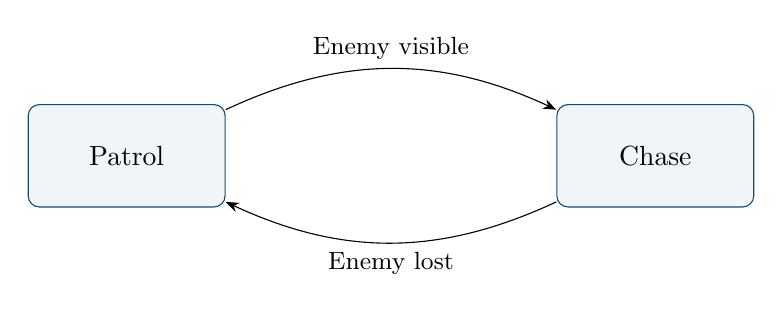
\begin{tikzpicture}[node distance=42mm]
\node[draw=vveblue,rounded corners,fill=vvelight,minimum width=25mm,minimum height=13mm] (p) {Patrol};
\node[draw=vveblue,rounded corners,fill=vvelight,minimum width=25mm,minimum height=13mm,right=of p] (c) {Chase};
\draw[-{Stealth},bend left=25] (p) to node[above,font=\small] {Enemy visible} (c);
\draw[-{Stealth},bend left=25] (c) to node[below,font=\small] {Enemy lost} (p);
\end{tikzpicture}\end{center}

Make state meanings clear. Patrol follows a patrol route; chase follows the player's estimated position; return moves back to a home point. A state should not mean an ambiguous mixture of unrelated activities. You can begin with two states and add a third only when a clear game rule needs it.

The VGAI state machine is a simple flat machine. It does not automatically provide nested states, parallel regions, a visual editor or saved-state serialization. You can still build useful behaviour by keeping perception, conditions and state actions small and explicit.
\lesson{A complete patrol and chase machine}
% doc-example: vgai_states_manual
\begin{lstlisting}
#include <cfloat>
#include <cmath>
#include <cstdint>
#include <limits>
#include "ViennaGameAILibrary.hpp"

int main() {
    bool enemyNear = false;
    int patrolUpdates = 0, chaseUpdates = 0;
    VGAIL::StateMachine machine;
    auto* patrol = machine.createState();
    auto* chase = machine.createState();
    patrol->onUpdateCallback = [&](float) { ++patrolUpdates; };
    chase->onUpdateCallback = [&](float) { ++chaseUpdates; };
    patrol->addTransition(chase, [&] { return enemyNear; });
    chase->addTransition(patrol, [&] { return !enemyNear; });
    machine.update(0.1f);
    enemyNear = true;
    machine.update(0.1f);
    enemyNear = false;
    machine.update(0.1f);
    const bool ok = patrolUpdates == 2 && chaseUpdates == 1
                && machine.getCurrentState() == patrol;
    std::cout << "states ok=" << ok
              << " patrol=" << patrolUpdates
              << " chase=" << chaseUpdates << '\n';
    return ok ? 0 : 1;
}
\end{lstlisting}
The three updates make the transition order observable. First patrol updates. Then enemy detection becomes true and chase updates. Finally it becomes false and patrol updates again. The expected totals are two patrol updates and one chase update. The machine owns both states until its destructor runs.
\lesson{Entry, transition, update and exit order}
On the first update, the machine chooses the first state created and calls its entry callback if present. It then scans that state's outgoing transitions in insertion order. The first true condition wins. It calls the old state's exit callback, chooses the target and calls the target's entry callback.

After those checks, it invokes the current state's update callback with dt. If a transition happened, this is the new state's update during the same call. The implementation makes at most one transition in that pass; it does not automatically chase every true transition through a chain of states.

Entry work is a good place to choose a route or reset a state-local timer. Update work advances the route or timer. Exit work can stop a sound or remove an activity-specific request. Keep gameplay changes explicit so changing callback order does not silently duplicate actions.

Conditions should generally report facts without side effects. If asking whether an enemy is near also removes the enemy or changes health, scanning priorities becomes difficult to reason about. Put the action in entry or update work, and keep the predicate a clear yes-or-no question.
\source{include/ViennaGameAILibrary.hpp: StateMachine::update; State::addTransition}
\lesson{Priorities, timers and stable behaviour}
If both low-health and enemy-visible conditions are true, whichever transition was added first wins. Put deliberate priority into the construction order and document it beside the setup. A useful test sets both conditions true and checks the chosen state. Do not depend on the reader guessing that order.

Add a timer by storing seconds in your game data and incrementing it during a state's update. Reset it in entry work. A predicate can check whether it exceeds a threshold. Remember that transitions are evaluated before update, so a threshold crossed during this update will normally affect the following call.

Repeated switching can happen when one noisy distance threshold controls both directions. For example, chase begins below ten metres and stops above ten. Small movement near ten can cause rapid changes. Use different thresholds, such as begin below nine and stop above eleven, or require a condition to remain true for a short duration.

Keep perception updates before state-machine updates in your frame. Then every transition in that call sees the same current facts. If state actions change shared perception data halfway through, record that policy deliberately or defer the changes until a later phase.
\lesson{Own states and captures safely}
\api{createState()} allocates and registers a state owned by the machine. The returned pointer is borrowed for configuration and observation. Do not manually delete it, transfer it to another owning machine or use it after the machine is destroyed. A state's transitions are also owned internally.

The current owning classes do not implement safe deep-copy semantics. Treat populated state machines, decision trees and flocks as non-copyable in game design, even though the compiler may accept an accidental copy. Store them in a stable owner such as a game scene or a \api{unique_ptr} and pass references where needed.

Callbacks can capture game data by reference. That makes conditions reflect current data instead of a copied initial value, but the referenced data must outlive all possible callback calls. Declare the game data before the machine in a simple scope so it remains alive while the machine is used and destroyed.

Avoid capturing a temporary local variable during setup and then saving the machine elsewhere. Prefer a reference to an owning agent object with a clear lifetime. If an agent can be removed, stop updating its machine before releasing any state data or render handles used by callbacks.
\source{include/ViennaGameAILibrary.hpp: State destructor; StateMachine destructor; Transition}
\lesson{Decision trees: follow questions to an action}
A decision tree asks a sequence of questions. If health is low, retreat; otherwise, if an enemy is near, attack; otherwise patrol. Each question chooses a branch, and a leaf performs an action. Unlike a state machine, a basic decision-tree evaluation does not by itself remember an active behaviour between calls.

VGAI supplies the ownership and call structure. Your derived nodes implement \api{makeDecision(float dt)}. A question node chooses a child and calls its \api{makeDecision}. A leaf does the requested work. The library does not automatically interpret a boolean condition or label a left branch true.

\begin{center}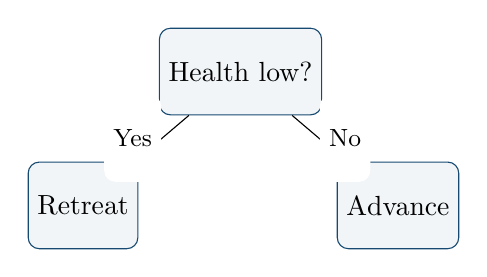
\begin{tikzpicture}[every node/.style={draw=vveblue,rounded corners,fill=vvelight,align=center,minimum height=11mm}]
\node (q) {Health low?};\node (a) at (-2,-1.7) {Retreat};\node (b) at (2,-1.7) {Advance};
\draw[-{Stealth}] (q)--node[draw=none,fill=white,left,font=\small] {Yes} (a);
\draw[-{Stealth}] (q)--node[draw=none,fill=white,right,font=\small] {No} (b);
\end{tikzpicture}\end{center}

Choose child ordering explicitly. In the next example, child 0 is retreat and child 1 is advance. The question node requires exactly those choices. A missing child or invalid index is a programming error; validate the setup before updates rather than expecting a fallback action to be invented.

A tree can choose a high-level request such as retreat while a separate movement layer executes it. That keeps a leaf small and avoids mixing route search, physical movement, animation and damage into one function.
\lesson{A complete decision tree}
% doc-example: vgai_tree
\begin{lstlisting}
#include <cfloat>
#include <cmath>
#include <cstdint>
#include <limits>
#include "ViennaGameAILibrary.hpp"

struct ActionLeaf : VGAIL::DecisionNode {
    int& count;
    explicit ActionLeaf(int& value) : count(value) {}
    void makeDecision(float) override { ++count; }
};
struct HealthChoice : VGAIL::DecisionNode {
    bool& low;
    explicit HealthChoice(bool& value) : low(value) {}
    void makeDecision(float dt) override {
        getChild(low ? 0 : 1).makeDecision(dt);
    }
};
int main() {
    bool lowHealth = true;
    int retreats = 0, advances = 0;
    VGAIL::DecisionTree tree;
    auto& root = tree.createRoot<HealthChoice>(lowHealth);
    root.addChild<ActionLeaf>(retreats);
    root.addChild<ActionLeaf>(advances);
    tree.update(0.1f);
    lowHealth = false;
    tree.update(0.1f);
    const bool ok = retreats == 1 && advances == 1;
    std::cout << "tree ok=" << ok << '\n';
    return ok ? 0 : 1;
}
\end{lstlisting}
The root selects retreat once and advance once. Each leaf increments a counter so branch choice can be verified without graphics. \api{createRoot} owns the root; \api{addChild} creates owned children. Keep only borrowed references for configuration. Replacing the root deletes its old descendants and invalidates references to them.
\lesson{Choose a tree or a state machine}
Use a state machine when a continuing activity matters. A reload animation, a patrol leg or a search timer naturally belongs to an active state. Entry and exit callbacks make start and stop actions explicit. A state remains active until a transition condition says otherwise.

Use a decision tree when you want to re-evaluate a set of questions and choose an action request. A tree can answer a tactical question each update using current facts. Repeated evaluation is useful, but an action that must happen only once needs its own state or event handling.

The approaches can cooperate. A state machine chooses combat mode; a small decision tree chooses a target or action within combat. Avoid adding both just because they are available. Begin with the simpler structure that expresses the behaviour clearly and test its priorities.

Neither facility is a behaviour-tree framework with built-in running, success and failure statuses. If you need long-running tasks, your game must represent that state deliberately. Naming the distinction helps prevent assumptions imported from another engine's AI tools.
\clearpage\part{Movement and groups}\lesson{Steering changes velocity}
Steering chooses how an agent should change its movement now. It can seek a target, flee from a threat or adjust toward nearby agents. A route planner chooses a larger-scale sequence of places. Combining them is useful: the planner supplies the next waypoint and steering moves toward it.

A \api{Boid} stores position, velocity, speed limits and a few movement values. It does not own a visible character or a physics body. You can inspect its position and copy it into your renderer, or use a desired velocity as input to your character controller.

The current \api{applySteeringForce} adds the supplied vector directly to velocity. Despite its name, that function does not multiply by elapsed time or divide by mass. If you treat the steering result as acceleration, multiply it by dt yourself before applying it.

\api{updatePosition(dt)} limits speed and advances position by velocity times dt. Apply acceleration once and move once per simulation update. Updating position twice or applying acceleration once per render frame with no dt conversion makes behaviour depend on the frame schedule.
\source{include/ViennaGameAILibrary.hpp: Boid::applySteeringForce; updatePosition}
\lesson{A complete seeking agent}
% doc-example: vgai_steering_manual
\begin{lstlisting}
#include <cfloat>
#include <cmath>
#include <cstdint>
#include <limits>
#include "ViennaGameAILibrary.hpp"

int main() {
    VGAIL::Boid agent({0.0f, 0.0f}, {0.0f, 0.0f}, 2.0f);
    const float dt = 0.1f;
    const VGAIL::Vec2f target{10.0f, 0.0f};
    for (int step = 0; step < 10; ++step) {
        auto acceleration = agent.seek(target, 1.0f);
        agent.applySteeringForce(acceleration * dt);
        agent.updatePosition(dt);
    }
    const auto p = agent.getPosition();
    const bool ok = std::isfinite(p.x) && p.x > 0.0f
                && std::abs(p.y) < 0.0001f;
    std::cout << "steering ok=" << ok
              << " x=" << p.x << " y=" << p.y << '\n';
    return ok ? 0 : 1;
}
\end{lstlisting}
After ten 0.1-second updates, the agent has moved to the right while staying on y = 0. The check does not require exact decimal output. It checks the movement direction and finite coordinates. Try changing dt and the number of updates while keeping the same total simulated time, and compare the difference caused by discrete integration.
\lesson{Seeking, fleeing and arriving}
\api{seek(targetPosition,maxAcceleration)} points toward a target. \api{flee} points away from a threat. The magnitude parameter scales the requested steering. These are useful local directions; they do not inspect walls or automatically choose a route around them.

Seeking alone can overshoot a target and repeatedly turn back. Arrival behaviour reduces its requested motion near a target. The current signature is \api{arrive(targetPosition,slowRadius,maxAcceleration)}. A positive slow radius defines where slowing begins. Choose it in the same world units as positions and compare its effect at the intended speed.

Test a target on the x axis before trying arbitrary directions. Print distance to the target, speed and position each update. If distance keeps growing, verify the sign of the target-minus-position direction and the mapping from world coordinates to the screen.

When blending movement requests, keep units consistent. If each result is treated as acceleration, combine acceleration vectors, limit the result if needed, multiply by dt and apply once. If one source produces a desired velocity instead, convert it deliberately rather than adding it as if it had the same units.
\source{include/ViennaGameAILibrary.hpp: Boid::seek; flee; arrive}
\lesson{Pursuit, evasion and wandering}
\api{pursue(targetBoid,maxAcceleration,maxPrediction)} estimates a future target position using its current movement. Prediction helps an agent intercept instead of always chasing where the target used to be. The target pointer is borrowed and must be valid during the call.

\api{evade} uses the same general idea to move away from a predicted threat. Prediction is limited by the chosen horizon. A target that changes direction suddenly can defeat the estimate; that is expected for a simple local model. Test a steady-moving target first, then introduce turns.

\api{wander(circleDistance,circleRadius,displacementRange,maxAcceleration)} creates changing local steering through a projected circle and a changing direction. It is useful for varied idle motion. It is random, so do not use one exact wandered position as a deterministic regression expectation.

These behaviours do not create map-aware navigation. A wandering agent still needs containment or collision rules if it must remain inside a room. A pursuer still needs a route when a wall separates it from the target. Local prediction cannot see through missing world information.
\source{include/ViennaGameAILibrary.hpp: Boid::pursue; evade; wander}
\lesson{What flocking tries to do}
Flocking combines several local influences. Separation encourages agents to avoid crowding. Alignment encourages them to move in similar directions. Cohesion encourages a group to stay together. A convincing group can emerge even when no agent has a complete plan for the flock.

The separation range is the nearby area used for avoiding close neighbours. The perception range is the wider neighbourhood used for matching and centring. Choose both in world units and make perception at least large enough to include the neighbours you expect agents to notice.

The parameters passed to \api{Flock::update} scale avoidance, matching and centring. They are tuning controls for this implementation, not a promise of a specific biological model. Start with a few explicitly placed agents and low factors, then add more only after the motion is understandable.

Flocking is also not collision avoidance with guaranteed clearance. Boids can overlap, cross walls or leave your play area without additional game rules. Add boundaries and collision handling at the movement layer when needed, and show perception ranges in a debug view while tuning.
\lesson{A complete two-agent flock}
% doc-example: vgai_flock
\begin{lstlisting}
#include <cfloat>
#include <cmath>
#include <cstdint>
#include <limits>
#include "ViennaGameAILibrary.hpp"

int main() {
    VGAIL::Flock flock;
    flock.addBoid({0.0f, 0.0f}, {1.0f, 0.0f}, 0.1f, 2.0f);
    flock.addBoid({1.0f, 0.2f}, {1.0f, 0.0f}, 0.1f, 2.0f);
    flock.setRanges(0.4f, 3.0f);
    for (int step = 0; step < 20; ++step)
        flock.update(0.05f, 0.1f, 0.05f, 0.01f);
    bool ok = flock.boids.size() == 2;
    for (auto* boid : flock.boids) {
        const auto p = boid->getPosition();
        ok = ok && std::isfinite(p.x) && std::isfinite(p.y);
    }
    std::cout << "flock ok=" << ok
              << " count=" << flock.boids.size() << '\n';
    return ok ? 0 : 1;
}
\end{lstlisting}
The test checks count and finite output after a bounded sequence. \api{Flock} owns the agents created by \api{addBoid}; its destructor deletes them. Do not also delete the pointers in \api{boids}, and do not insert pointers to stack objects into that owning vector.
\lesson{Read the current flocking formulas carefully}
The standalone steering helpers and the combined flock update have different details. In the standalone \api{separation} helper, the loop replaces its result for each nearby neighbour instead of accumulating every contribution. The final neighbour visited can therefore influence that helper's result disproportionately. The combined \api{doFlocking} path used by \api{Flock::update} accumulates separation contributions.

The standalone \api{cohesion} helper subtracts the boid's velocity from the average neighbour position. Those quantities have different meanings; a conventional cohesion vector would compare positions. The combined flock update does compare positions for its centring contribution. Keep those paths distinct when interpreting tuning results. This guide documents the source; updating algorithms would be a separate code change with its own tests.

The combined update adjusts velocity using its factors directly, then multiplies velocity by dt to advance position. Its factors are therefore tied to update frequency rather than automatically representing per-second acceleration. Use a fixed update interval when tuning. A zero-speed boid with a positive minimum speed can also enter a division by zero in that path; initialize meaningful nonzero velocities or choose and test a game-side policy for stationary agents.

The flock also updates boids in place, in vector order. A later boid can see earlier boids after they have moved in the same update. A simultaneous model would first read an unchanged snapshot and then apply all results. The current ordering can make output depend on insertion order.

Use small numerical experiments before relying on emergent motion: one neighbour, two symmetric neighbours, reversed insertion order and no neighbours. Record velocities as well as positions. These tests help distinguish tuning from the actual formulas used by your source version.
\source{include/ViennaGameAILibrary.hpp: Boid::separate; align; cohesion; doFlocking; Flock::update}
\lesson{Let one system own the final position}
If both a boid and a rigid body independently advance position, they can disagree. Decide which system produces final movement. For a simple top-down console or raylib demo, the boid can own movement and the renderer simply copies its position.

For a physical character, use AI to choose a desired velocity or movement request. The physics or character controller applies allowed movement, including collision response. Feed the resulting position back into the AI's representation before the next decision. Do not overwrite physics with a second unconstrained position every frame.

In a 3D renderer, map the two AI coordinates to the intended ground-plane axes. For example, AI x and y may map to world x and z, while world y remains height. Rotation derived from two-dimensional velocity must use that same convention.

Test a wall in a small scene. First confirm the AI wants to move toward the goal. Then confirm the collision layer stops unsafe movement. Finally confirm the renderer follows the accepted position. This order keeps a visual mapping mistake from looking like a pathfinding failure.
\clearpage\part{Trying possible futures}\lesson{Monte Carlo tree search without the jargon}
Some decisions are best judged by trying possible futures. In a turn-based game, the AI can copy the current board, try a legal move, simulate more moves and see who wins. Repeating this process gives evidence about which first move is promising. Monte Carlo refers to the random trial choices used in those simulations.

Tree search stores alternatives in a branching structure. A node represents a game state. An edge represents an action leading to another state. A visit count records how often the search explored that node, and result counts help compare alternatives.

The method balances exploitation, choosing something that has worked well, with exploration, trying less-tested alternatives. A parameter controls that balance. More search time can improve evidence, but it does not guarantee the strongest move in every position.

Use MCTS only when you can cheaply copy game state and simulate legal actions without changing the live game. Do not use a renderer object or an entire active physics world as a casual copyable state. Start with a tiny finite board or token game where every trial eventually ends.
\lesson{The four search phases}
\textbf{Selection}: walk through already explored alternatives using their statistics until reaching a place that should be expanded or evaluated. The current implementation uses an upper-confidence style comparison, combining estimated success with an exploration term.

\textbf{Expansion}: choose an untried legal action, copy the state and execute that action on the copy. A new child stores the result. Your action must update the state's legal-action list and terminal status correctly.

\textbf{Simulation}: continue with randomly chosen legal actions until a terminal result or no legal actions remain. This implementation's rollout has no separate depth or duration limit. Your game model must guarantee that trial play finishes; the outer search budget cannot interrupt an endless rollout.

\textbf{Backpropagation}: walk back up the parent chain and update visit and result counts. Once the outer budget ends and workers join, the current root chooses the child with the greatest visit count.

Search quality depends strongly on the correctness of your state and action implementation. If illegal actions remain listed, a winner is reported too early or a copied state shares live mutable game data, the statistics can be meaningless even when the search returns an action.
\source{include/ViennaGameAILibrary.hpp: MCTS::select; expand; simulate; backpropagate; runMCTS}
\lesson{Define the state and action contract}
Your action type can derive from \api{Action<YourState>} and implement \api{execute(YourState&)}. It changes the supplied state. It should not mutate the live board through an external pointer or draw a frame. Actions should be ordinary copyable values representing choices such as a cell index.

Your state can derive from \api{MCTSState<YourState,YourAction>}. It carries legal actions, terminal status, the player whose turn it is and the winner ID. Its constructor initializes those values. Every action must keep them consistent after execution. The action list is the next state's available choices, not a log of moves already taken.

A state is copied many times. A copy must be independent for simulated changes. A \api{std::vector} of board values is a straightforward choice; a pointer to one shared mutable board is usually not. Keep the state small enough that trial play is affordable.

Player identifiers are strings in this implementation. Use a consistent spelling for each player across turns and results. Define what a draw means in your model and inspect how the implementation counts winners; do not assume an automatic half-point draw reward or a general multi-player utility model.
\source{include/ViennaGameAILibrary.hpp: Action; MCTSState; MCTSNode}
\lesson{A complete MCTS contract exercise}
This deliberately tiny game has one legal move, and that move ends the game with player A winning. It verifies that custom state and action types satisfy the actual template API. It is not a comparison of search strength.% doc-example: vgai_mcts
\begin{lstlisting}
#include <cfloat>
#include <cmath>
#include <cstdint>
#include <limits>
#include "ViennaGameAILibrary.hpp"

struct Turn;
struct Move : VGAIL::Action<Turn> {
    void execute(Turn& state) override;
};
struct Turn : VGAIL::MCTSState<Turn, Move> {
    Turn() : MCTSState(std::vector<Move>{Move{}}, false, "A") {}
    void finish() {
        actions.clear();
        isTerminal = true;
        winnerPlayerId = "A";
    }
};
void Move::execute(Turn& state) { state.finish(); }

int main() {
    Turn start;
    VGAIL::MCTS<Turn, Move> search;
    // One legal action, positive milliseconds, one worker.
    Move chosen = search.runMCTS(start, 20.0, 1.0, 1);
    chosen.execute(start);
    const bool ok = start.getIsTerminal()
                 && start.getWinnerPlayerId() == "A";
    std::cout << "mcts_contract ok=" << ok << '\n';
    return ok ? 0 : 1;
}
\end{lstlisting}
Expected result: \api{mcts_contract ok=1}. The search budget is 20 milliseconds and the worker count is one. A larger game should handle a terminal state, no legal moves or exactly one legal move directly before starting a search.
\lesson{Budgets, randomness and input preconditions}
\api{runMCTS(state,timeLimitMs,c,thread_count)} uses milliseconds for its budget. Use a positive budget and at least one worker. The current implementation assumes a best child exists when returning; a terminal root, no legal actions or a zero-duration search can leave that pointer empty. Guard those cases in your game before calling it.

For one legal move, return that move directly in production game code. For several moves, a positive budget is a practical precondition, not an absolute guarantee that a worker runs before its deadline on every overloaded machine. A robust application integration needs a fallback policy around this API if that risk matters.

The budget is checked between search iterations. One expensive rollout can run beyond it. A rollout can also fail to terminate if your game permits endless repeated positions without a draw or repetition rule. Add finite terminal rules to the game model and test them independently of MCTS.

Rollouts choose random actions and the amount of work depends on elapsed wall time. Do not assert one exact selected move or visit count as a general deterministic test. Check that the returned action is legal, that its execution changes a copied state correctly and that the live state was not mutated during search.

Start with one worker. The implementation contains mutexes and atomics, but those alone do not establish that every user state, callback and shared container is safe for arbitrary concurrent access. Add concurrency only after examining the actual access paths and measuring a benefit.
\source{include/ViennaGameAILibrary.hpp: MCTS::runMCTS; searchBestAction; simulate}
\lesson{A complete finite token game}
Two players take one or two of five tokens each turn. Taking the last token wins. The code refreshes legal actions and changes players after each nonterminal action. Every trial finishes because the token count decreases. Search copies the state; only the selected action is later applied to the live game.% doc-example: vgai_take_game
\begin{lstlisting}[basicstyle=\ttfamily\footnotesize]
#include <cfloat>
#include <cmath>
#include <cstdint>
#include <limits>
#include "ViennaGameAILibrary.hpp"

struct Game;
struct Take : VGAIL::Action<Game> {
    int count = 1;
    Take() = default;
    explicit Take(int value) : count(value) {}
    void execute(Game& state) override;
};
struct Game : VGAIL::MCTSState<Game, Take> {
    int remaining = 5;
    Game() : MCTSState({}, false, "A") { refreshActions(); }
    void refreshActions() {
        actions.clear();
        for (int n = 1; n <= 2 && n <= remaining; ++n)
            actions.emplace_back(n);
    }
    void take(int n) {
        remaining -= n; // The caller supplies only legal moves.
        if (remaining == 0) {
            isTerminal = true;
            winnerPlayerId = playerTurnId;
        } else {
            playerTurnId = playerTurnId == "A" ? "B" : "A";
        }
        refreshActions();
    }
};
void Take::execute(Game& state) { state.take(count); }

int main() {
    Game live;
    VGAIL::MCTS<Game, Take> search;
    Take chosen = search.runMCTS(live, 20.0, 1.0, 1);
    const bool legal = chosen.count >= 1 && chosen.count <= 2;
    const bool unchanged = live.remaining == 5;
    if (legal)
        chosen.execute(live);
    const bool ok = legal && unchanged
                 && live.remaining == 5 - chosen.count;
    std::cout << "take_game ok=" << ok
              << " chosen=" << chosen.count
              << " remaining=" << live.remaining << '\n';
    return ok ? 0 : 1;
}
\end{lstlisting}
Expect \api{take_game ok=1} and a chosen count of 1 or 2. The check validates legality, state independence and execution. It deliberately does not assert that this short random search always selects a game-theoretically best move. Test action rules separately before using search results to judge strategy.
\clearpage\part{Putting the parts into a game}\lesson{A clear frame order}
Begin by gathering facts: positions accepted by movement, visible targets, health, door states and the current navigation map version. Then evaluate behaviour decisions. A state machine or tree can choose a goal or action request using those facts.

Next update route requests that need refreshing. Follow existing waypoints and calculate desired movement. Apply allowed movement through your character controller or physics integration. Finally copy accepted positions and animation requests to the renderer. Handle removals at a point where no callback or loop is still using the removed object.

You do not need every subsystem at the same rate. Decisions might run ten times per second while movement runs at a fixed simulation rate and rendering runs as often as possible. Use measured durations and stored state between updates. Do not accidentally pass render-frame dt to a decision timer that is called less often.

Keep a simple single-agent scene first. Print current state, target cell, route index, desired velocity and accepted position. Those five values identify most integration mistakes more quickly than adding many debug arrows to an already crowded scene.
\lesson{Connect VGAI, VPE and VVE}
The three projects can cooperate through your game code. VGAI chooses behaviour and desired motion. VPE calculates physical response for bodies and cloth. VVE draws visible objects and provides the application-facing engine facade. Each library keeps its own role.

Use a stable game object or entity record as the association point. It can hold the AI state, the physics body reference and a public VVE render-object handle. Avoid making AI depend on a concrete VVE implementation namespace or storing internal renderer descriptors inside search states.

For a guard on a ground plane, map the two AI coordinates to physical x and z. Let AI request a horizontal direction or velocity, then let physics apply it according to the game's movement rules. Read back the resulting position before the next AI decision. Copy the accepted pose to VVE through its official facade.

An MCTS state should remain a separate small game-rule model. Copying it must not copy or mutate the active render scene or physical simulation. If a search action means move to cell 4, the live game executes that chosen action later through its normal systems.

Unit conversions belong at the boundary. Grid cells, world metres, pixels, seconds and search milliseconds are distinct. Name those values clearly and test one round trip between cell coordinates and world coordinates before adding a large map.
\lesson{Test claims with small reproducible inputs}
For paths, use zero random obstruction, explicit blocked cells and known endpoints. Check start and finish, valid adjacency, walkability and the unreachable case. Add a blocked-corner case so the chosen diagonal policy is visible in your test expectations.

For state machines, record entry, exit and update events in a vector. Check the first update, one transition, simultaneous true predicates and a timer threshold. The expected event order matters as much as the final active pointer.

For decision trees, count which leaves ran under each condition. Check that every branch exists before updating. For steering, use a fixed dt and a target on one axis; check finite output and movement direction. For flocks, test empty and small groups, symmetric placements and reversed insertion order.

For MCTS, first test actions and copied states directly without a search. Ensure trial play ends and all reported legal actions really are legal. Then check that the search returns an allowed action and leaves the live input unchanged. Treat quality comparisons as measured experiments over many positions and runs.

Print small named fields such as \api{path_ok=1}, dimensions, route size, update counts and the first failing step. Return nonzero for a failed condition. This makes console examples useful to people, CI jobs and automated debugging tools without requiring image interpretation.
\lesson{Performance: measure the right work}
For pathfinding, distinguish map construction, preprocessing and query latency. Report map dimensions, obstacle arrangement and query count. A faster preprocessed query may still lose overall if the map changes so often that caches are constantly rebuilt.

For many agents, count searches per second rather than only agents on screen. Reusing an unchanged route and staggering requests can reduce repeated work. Make any route cache depend on the goal and map version so it cannot silently return a path through a newly closed door.

For flocking, neighbour comparisons can grow quickly as groups grow. Measure the current implementation before introducing a spatial index or parallel update. An algorithm change also needs tests for ordering and simultaneous-versus-sequential semantics; performance is not the only consequence.

For MCTS, separate state-copy cost, legal-action generation, rollout length and total search budget. A tiny compact state can allow more useful trials than a large object graph. Increase the budget only after confirming the game model is correct and the response time is acceptable.

The current \api{NavMesh} owns allocated region structures whose cleanup should be reviewed before repeatedly constructing and destroying many maps in a long-lived process. The guide does not change library ownership code. Profile and test the lifetime pattern your game actually uses.
\source{include/ViennaGameAILibrary.hpp: NavMesh destructor; region storage; Flock::update; MCTS}
\lesson{Troubleshooting from symptom to cause}
\textbf{The header does not compile on Linux}: confirm C++20 mode, required standard headers and the current debug-assertion path. The console examples define \api{NDEBUG}. A missing \api{__debugbreak} is an assertion portability issue, not a pathfinding configuration problem.

\textbf{Duplicate symbols at link time}: check whether several source files include the current implementation header. Keep a single integration source file or make a separately reviewed change to the header's linkage design.

\textbf{No route}: check bounds, endpoint walkability and the complete barrier layout. \textbf{A route cuts a blocked corner}: inspect the diagonal-neighbour rule. \textbf{A character ignores the route}: check world-to-cell conversion and waypoint advancement.

\textbf{The wrong state wins}: inspect transition insertion order and whether the condition facts were updated before the machine. \textbf{A state changes one update later}: remember that transitions are checked before the state's update callback.

\textbf{Motion changes with frame rate}: check where dt is multiplied, how often movement runs and whether acceleration is applied once. \textbf{A boid crosses a wall}: add or inspect collision handling; steering is only a movement request.

\textbf{A search hangs}: verify that simulated play reaches a terminal result and does not repeat indefinitely. \textbf{MCTS crashes immediately}: check terminal state, legal moves, positive budget and worker count before entering \api{runMCTS}. \textbf{A crash follows scene deletion}: inspect captured references and ownership before changing algorithms.
\lesson{A small reference and a sensible next project}
\textbf{Create a map}: \api{NavMesh(width,height,obstacleFraction)}. \textbf{Change cells}: \api{setObstructable} and \api{setWalkable}. \textbf{Find a route}: \api{findPath(start,target)}. \textbf{Prepare cached routing}: \api{preprocess}, then \api{findPreprocessedPath} on the matching map.

\textbf{Remember a behaviour}: create a \api{StateMachine}, call \api{createState}, assign callbacks, add transitions and call \api{update(seconds)}. \textbf{Choose through questions}: derive \api{DecisionNode}, create a root, add children and implement \api{makeDecision}.

\textbf{Move one agent}: create a \api{Boid}, compute steering, convert acceleration to a velocity change with dt, then call \api{updatePosition(dt)}. \textbf{Move a group}: create a \api{Flock}, add boids, set ranges and call \api{update} with measured seconds and tuning factors.

\textbf{Try future actions}: provide copyable game state and action types, handle terminal and trivial cases in your game, then call \api{MCTS<State,Action>::runMCTS} with a positive millisecond budget. Execute the selected action on the live game only after the search returns.

A good first integrated project is one guard in a small grid room. It patrols between two points, chases a visible target and returns home. Keep routes visible, print its state and use a collision-aware movement layer. Add a second guard only after the first behaves correctly. This gives every algorithm a clear job and leaves you with tests you can reuse.
\source{include/ViennaGameAILibrary.hpp; Demo/src; README.md}

\end{document}
